\subsection{Hipoteza i metoda weryfikacji}

Hipoteza badawcza pracy, sformułowana w sekcji~1.1, brzmi:

\begin{quote}
\emph{Zastosowanie indeksów znacząco poprawia wydajność operacji SELECT
kosztem spadku wydajności operacji INSERT i UPDATE.}
\end{quote}

Hipoteza ma dwie części, których każda wymaga osobnej weryfikacji.
W pierwszej (sekcja 13.2) sprawdzamy, czy operacje czytające faktycznie
zyskują na obecności indeksów dodatkowych. W drugiej (sekcja 13.3)
sprawdzamy, czy operacje zapisujące tracą. Dodatkowo (sekcja 13.4)
analizujemy operacje DELETE -- nieuwzględnione w pierwotnej hipotezie,
ale dające ciekawe wnioski.

Metryką weryfikacji jest \textbf{stosunek czasu wykonania z indeksami
do czasu wykonania bez indeksów} (medianowych), liczony osobno dla
każdej pary (scenariusz, silnik, wolumen). Wartość poniżej 1.0 oznacza,
że indeks przyspieszył operację (im niżej, tym mocniej); wartość
powyżej 1.0 oznacza spowolnienie; wartość około 1.0 -- brak istotnego
wpływu. Wizualnym podsumowaniem są trzy mapy cieplne -- po jednej
na wolumen -- pokazujące ten stosunek dla wszystkich 24 scenariuszy
i 4 silników.

\begin{figure}[H]
    \centering
    
\includegraphics[width=1.0\textwidth]{charts/small/index_heatmap_small.png}
    \caption{Mapa cieplna wpływu indeksów -- wolumen \emph{small}.
    Zielony = indeks przyspieszył, czerwony = spowolnił, żółty = brak
    istotnej różnicy.}
\end{figure}

\begin{figure}[H]
    \centering
    
\includegraphics[width=1.0\textwidth]{charts/medium/index_heatmap_medium.png}
    \caption{Mapa cieplna wpływu indeksów -- wolumen \emph{medium}.}
\end{figure}

\begin{figure}[H]
    \centering
    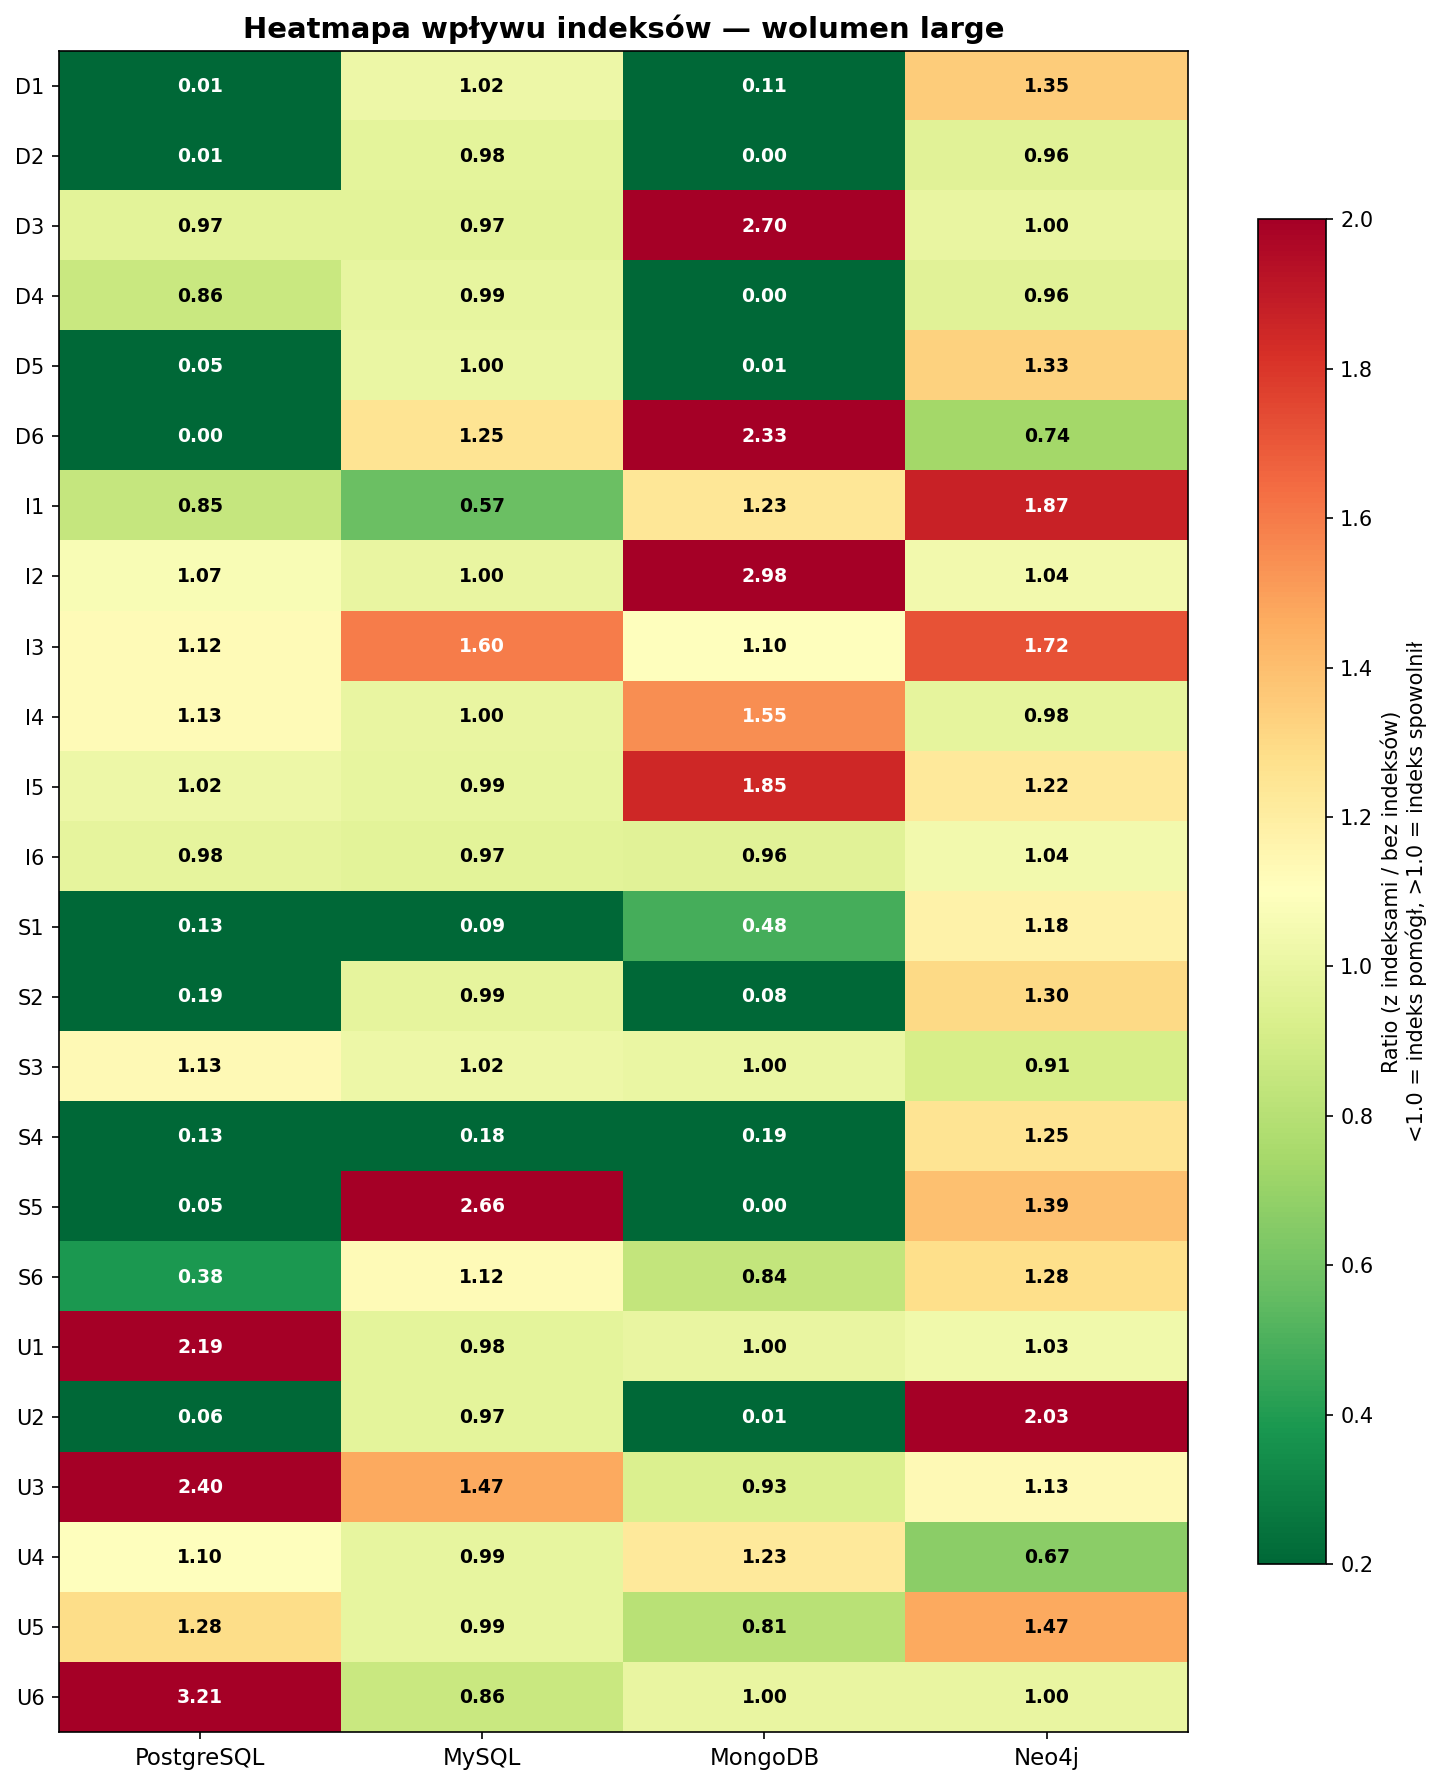
\includegraphics[width=1.0\textwidth]{charts/large/index_heatmap_large.png}
    \caption{Mapa cieplna wpływu indeksów -- wolumen \emph{large}.}
\end{figure}

% -------------------------------------------------------
\subsection{Część I -- wpływ indeksów na operacje SELECT}

W kategorii SELECT mamy 6 scenariuszy (S1--S6) wykonywanych na
4 silnikach i 3 wolumenach -- razem 72 punkty pomiarowe. Z map
cieplnych wynika, że \textbf{w zdecydowanej większości komórek
pierwsza część hipotezy się potwierdza}, ale obraz nie jest
jednorodny.

\subsubsection*{Scenariusze, w których indeks pomaga konsekwentnie}

Najsilniejsze potwierdzenia hipotezy pochodzą ze scenariuszy
\textbf{S1, S5 oraz S4}:

\begin{itemize}
    \item \textbf{S5 MongoDB} -- stosunek 0.03 / 0.03 / 0.00 (czyli
    redukcja czasu o 97--99.5\%) na trzech wolumenach. Bez indeksu
    silnik wykonuje \texttt{COLLSCAN} po milionach dokumentów,
    z indeksem trafia od razu w 12--25 rekordów.
    \item \textbf{S1 MySQL} -- 0.59 / 0.27 / 0.09 -- coraz większa
    poprawa wraz z rozmiarem tabeli, czyli wzór dokładnie zgodny
    z hipotezą: indeks zyskuje na wartości tym bardziej, im więcej
    danych trzeba pominąć.
    \item \textbf{S4 wszystkie silniki na medium} -- ratio 0.14--0.47.
    Indeksy pełnotekstowe (GIN trigramowy w PG, \texttt{text} w Mongo,
    Lucene w Neo4j) drastycznie przyspieszają wyszukiwanie po
    fragmencie tekstu.
    \item \textbf{S2 PostgreSQL i MongoDB} -- ratio 0.04--0.52
    i 0.06--0.10 odpowiednio.
\end{itemize}

\subsubsection*{Główny wyjątek: S3}

S3 (TOP 100 z ostatnich miesięcy) jest jedynym scenariuszem
SELECT, w którym indeks praktycznie nie pomaga w żadnym
silniku -- ratio waha się 0.84--1.18. Wyjaśnienie znane z analizy
EXPLAIN (sekcja 11.3): filtr po dacie \texttt{started\_at} obejmuje
tak duży podzbiór wierszy, że nawet bitmapowy odczyt z indeksu
i tak musi sięgnąć po większość stron tabeli. To pokazuje
\textbf{granicę zastosowalności hipotezy}: indeks przyspiesza
SELECT-y wtedy, gdy filtr jest wystarczająco selektywny.

\subsubsection*{Specyficzne ograniczenia poszczególnych silników}

\textbf{Neo4j} zachowuje się odmiennie od pozostałych baz. Dla S1
oraz S2 stosunek nie spada poniżej 0.5, a dla S5 na \emph{large}
przekracza nawet 1.0. Wyjaśnienie znane z 11.3: w grafie kluczowe
indeksy istnieją już jako ograniczenia unikalności (\texttt{:Genre.name},
\texttt{:Person.person\_id}), więc baseline ,,bez indeksów'' jest
częściowo zindeksowany.

\textbf{MySQL} wykazuje analogiczny artefakt -- indeksy chroniące
klucze obce nie dają się usunąć (sekcja 11.1), więc pomiar
,,bez indeksów'' nie jest w pełni czysty. Mimo tego dla S1 i S4
ratio jest wyraźnie poniżej 1.0.

\subsubsection*{Werdykt części I}

Hipoteza w części dotyczącej SELECT jest \textbf{potwierdzona
zdecydowaną większością przypadków}. W 4 z 6 scenariuszy (S1, S2,
S4, S5) co najmniej 2 z 4 silników osiągają ratio poniżej 0.5 na
\emph{medium} i \emph{large}. Dwa istotne zastrzeżenia, z którymi
hipoteza się musi zmierzyć: \emph{niska selektywność} (S3) oraz
\emph{architektura silnika} (Neo4j i częściowo MySQL).

% -------------------------------------------------------
\subsection{Część II -- wpływ indeksów na operacje INSERT i UPDATE}

W kategorii INSERT i UPDATE mamy łącznie 12 scenariuszy
(I1--I6, U1--U6). Hipoteza przewiduje wzrost czasu wykonania -- czyli
ratio powyżej 1.0. Z danych wynika, że \textbf{ten kierunek jest
potwierdzony, ale w postaci wyraźnie słabszej niż dla SELECT-ów}.

\subsubsection*{Najmocniejsze dowody}

\begin{itemize}
    \item \textbf{U3 PostgreSQL} (masowa zmiana planu subskrypcji) --
    ratio 1.91 / 2.17 / 2.40, rosnący z wolumenem. To podręcznikowy
    przykład utrzymania indeksu \texttt{(status, plan\_name)} przy
    aktualizacji każdego z milionów wierszy.
    \item \textbf{U6 PostgreSQL} -- ratio 2.56 / 2.44 / 3.21 -- jeszcze
    silniejsza penalizacja niż U3. Operacja modyfikuje pole indeksowane
    w wielu wierszach.
    \item \textbf{I2 MongoDB} (bulk import ocen) -- ratio 3.08 / 2.39 / 2.98.
    Każdy nowy dokument musi zaktualizować strukturę indeksu B-drzewa,
    co u Mongo przekłada się na wyraźny narzut.
    \item \textbf{U1 PostgreSQL na large} -- ratio 2.19, przejście
    profilu na ,,kids'' -- każda aktualizacja dotyka indeksu na
    \texttt{is\_kids}.
\end{itemize}

\subsubsection*{Scenariusze obojętne}

W większości scenariuszy I1--I6 ratio waha się 0.85--1.15 -- czyli
bez wyraźnego wpływu w żadną stronę. Powód jest dwojaki. Po pierwsze,
część scenariuszy modyfikuje pojedyncze wiersze (np. I3 -- jeden
serial), więc narzut indeksu jest pomijalny. Po drugie, dla MySQL
i PostgreSQL koszt \texttt{INSERT}-a jest dominowany przez zapis WAL/redo
log, a nie przez utrzymanie indeksów dodatkowych.

\subsubsection*{Specyficzne anomalie}

W kilku komórkach map cieplnych pojawiają się wartości wyraźnie
poniżej 1.0 dla operacji zapisujących -- np. \textbf{U2 MongoDB
(0.15 / 0.05 / 0.01)} czy \textbf{U2 PostgreSQL (0.35 / 0.17 / 0.06)}.
Pozornie sprzeczne z hipotezą, ale wytłumaczalne: U2 ,,przelicza średnią
ocenę'' i \emph{najpierw} musi znaleźć właściwy wiersz/dokument
(operacja typu SELECT), \emph{dopiero potem} go zaktualizować.
Skoro filtr SELECT jest punktowy i indeks go drastycznie przyspiesza,
to dominujący koszt całej operacji spada -- nawet jeśli sam
\texttt{UPDATE} jest minimalnie droższy. To pokazuje, że hipoteza
w wersji ,,UPDATE jest zawsze wolniejszy z indeksem'' jest
\emph{zbyt mocna} -- prawdziwsza forma to: ,,operacja z punktowym
filtrem zyskuje na indeksie tak samo jak SELECT, niezależnie od tego,
czy kończy się modyfikacją''.

\subsubsection*{Werdykt części II}

Hipoteza w części dotyczącej INSERT/UPDATE jest \textbf{potwierdzona,
ale w postaci osłabionej}. Spowolnienie pojawia się tam, gdzie operacja
modyfikuje wiele wierszy w kolumnie indeksowanej (U3, U6, I2). Dla
operacji z punktowym filtrem hipoteza jest faktycznie \emph{odwracana} --
indeks pomaga, bo dominujący koszt jest po stronie wyszukiwania,
nie zapisu.

% -------------------------------------------------------
\subsection{Operacje DELETE poza hipotezą}

Operacje DELETE nie zostały uwzględnione w pierwotnej hipotezie, ale
pomiary pokazują wyrazisty wzorzec, który warto omówić.

\subsubsection*{Indeks pomaga -- spektakularnie}

Najsilniejszy wynik całej pracy pochodzi właśnie z DELETE:
\textbf{D6 PostgreSQL na large} -- ratio \textbf{0.00} (formalnie
0.0003) -- co w wartościach absolutnych oznacza spadek z 30.7~sekundy
do 10~milisekund. Tysiąckrotne przyspieszenie. Podobne efekty:

\begin{itemize}
    \item D1 PostgreSQL -- ratio 0.07 / 0.05 / 0.01 (skala rośnie
    z wolumenem -- na large 100-krotne przyspieszenie).
    \item D2 PostgreSQL -- 0.10 / 0.15 / 0.01.
    \item D5 PostgreSQL i MongoDB -- 0.43--0.05 i 0.09--0.01.
    \item D4 MongoDB -- 0.03 / 0.01 / 0.00 -- liniowe skalowanie
    skanu kolekcji bez indeksu, eliminowane przez \texttt{IXSCAN}.
\end{itemize}

\subsubsection*{Dlaczego DELETE działa jak SELECT}

Każde usunięcie poprzedzone jest \emph{wyszukaniem} wiersza/dokumentu
do usunięcia. Operacje masowe (D6 -- usuń wszystkich nieaktywnych
użytkowników) lub kaskadowe (D1 -- usuń treść wraz z powiązanymi)
wymagają znalezienia setek lub tysięcy wierszy zależnych. Bez indeksu
to seria pełnych skanów; z indeksem -- bezpośrednie trafienie.
Sama akcja usunięcia jest natomiast tania (przepisanie strony,
oznaczenie wiersza jako martwego).

\subsubsection*{Kontrprzykłady -- DELETE z indeksem może być wolniejszy}

W dwóch scenariuszach DELETE w MongoDB indeks paradoksalnie spowalnia:
\textbf{D3 MongoDB} (1.75 / 2.04 / 2.70) i \textbf{D6 MongoDB}
(1.42 / 1.82 / 2.33). Powodem są masowe usunięcia (\texttt{deleteMany})
po polu nieindeksowanym -- silnik przejdzie tabelę tak czy inaczej,
ale dla każdego usuwanego dokumentu musi dodatkowo zaktualizować
\emph{wszystkie} indeksy. To jest ten sam mechanizm, który widzieliśmy
w INSERT/UPDATE -- tylko że w odwrotnej fazie życia dokumentu.

\subsubsection*{Uogólnienie hipotezy}

DELETE pokazuje, że hipoteza dałaby się sformułować ogólniej:
\emph{indeks przyspiesza fazę wyszukiwania w dowolnej operacji
i spowalnia fazę modyfikacji w dowolnej operacji}. Czy operacja
zwraca wynik (SELECT), modyfikuje go (UPDATE), czy usuwa (DELETE) --
to drugorzędne. Liczą się dwie rzeczy: \emph{jak selektywny jest filtr}
i \emph{ile wierszy jest faktycznie modyfikowanych}.

% -------------------------------------------------------
\subsection{Werdykt per silnik}

Każdy z czterech silników w specyficzny sposób potwierdza lub
osłabia hipotezę. Tabela~\ref{tab:hypothesis_verdict} podsumowuje
zachowanie.

\begin{table}[H]
    \centering
    \small
    \begin{tabular}{lll}
        \toprule
        \textbf{Silnik} & \textbf{Część I (SELECT)} & \textbf{Część II (INSERT/UPDATE)} \\
        \midrule
        PostgreSQL & potwierdzona mocno    & potwierdzona mocno \\
        MySQL      & częściowo (FK index)  & częściowo \\
        MongoDB    & potwierdzona mocno    & potwierdzona (I2, częściowo U) \\
        Neo4j      & częściowo (constraint indexes) & słabo obserwowana \\
        \bottomrule
    \end{tabular}
    \caption{Werdykt weryfikacji hipotezy per silnik.}
    \label{tab:hypothesis_verdict}
\end{table}

\textbf{PostgreSQL} jest najbardziej ,,podręcznikowym'' przypadkiem.
Pełne potwierdzenie obu części hipotezy: ratio 0.05--0.13 dla
SELECT-ów na \emph{large} (S1, S2, S4, S5) oraz ratio 1.91--3.21 dla
problematycznych UPDATE-ów (U3, U6). Bogactwo typów indeksów
(częściowy, GIN trigramowy, GIN dla \texttt{jsonb}) wzmacnia
część pierwszą.

\textbf{MySQL} jest najtrudniejszy do oceny. Niemożliwość upuszczenia
indeksu chroniącego klucz obcy oznacza, że pomiar ,,bez indeksów''
jest częściowo skażony. Mimo tego dla SELECT-ów S1 i S4 ratio jest
wyraźnie poniżej 1.0 (0.09--0.27), a dla U3 i U6 powyżej 1.0
(1.36--1.47). Hipoteza więc się broni, choć bez tej dramatyzacji
co PG.

\textbf{MongoDB} jest najbardziej kontrastowym przypadkiem -- ze
względu na to, że w wariancie ,,bez indeksów'' faktycznie wykonuje
pełne skany kolekcji. Stąd najmocniejsze ratio części pierwszej
(S5: 0.00 na \emph{large}) i części drugiej (I2: 2.39--3.08).
Architektura dokumentowa wzmacnia obie strony hipotezy.

\textbf{Neo4j} najsłabiej potwierdza hipotezę -- co nie jest porażką
silnika, ale konsekwencją jego architektury. Ograniczenia unikalności
zakładane przy ładowaniu zapewniają indeksy dla najczęstszych dostępów,
więc baseline ,,bez indeksów'' jest już częściowo zoptymalizowany.
Część druga hipotezy w Neo4j prawie nie występuje -- modyfikacje
węzła i relacji nie wymagają wielu aktualizacji indeksów, bo grafy
mają tych indeksów mniej z natury.

% -------------------------------------------------------
\subsection{Wnioski końcowe}

Hipoteza pracy: \emph{,,zastosowanie indeksów znacząco poprawia
wydajność operacji SELECT kosztem spadku wydajności operacji INSERT
i UPDATE''} -- została \textbf{potwierdzona w postaci ogólnej},
z dwoma istotnymi zastrzeżeniami.

\textbf{Po pierwsze}, korzyść z indeksu jest funkcją \emph{selektywności
filtru}: indeks przyspiesza operację tym mocniej, im węższy podzbiór
wierszy zwraca filtr \texttt{WHERE}. Dla S3 (filtr po dacie obejmujący
1/6 tabeli) ratio pozostaje bliskie 1.0 niezależnie od silnika -- co
pokazuje granicę przydatności indeksu.

\textbf{Po drugie}, koszt indeksu dla operacji zapisującej zależy
nie tyle od samego typu operacji (INSERT vs UPDATE), co od
\emph{liczby modyfikowanych wierszy w kolumnie indeksowanej}. Dla
masowych \texttt{UPDATE}-ów po kolumnie indeksowanej (U3, U6) koszt
indeksu jest istotny (1.5--3×). Dla pojedynczych modyfikacji
po wyszukaniu wiersza (U2) -- indeks paradoksalnie pomaga, bo
dominujący koszt jest po stronie wyszukiwania.

\textbf{Praktyczna rekomendacja} wynikająca z badań: indeksy zakładać
agresywnie dla kolumn intensywnie filtrowanych w SELECT-ach
i DELETE-ach, ostrożnie dla kolumn często aktualizowanych masowo.
Najsilniejszy wpływ na wydajność systemu produkcyjnego mają indeksy
na kluczach obcych w tabelach uczestniczących w kaskadowym usuwaniu
oraz indeksy częściowe dla często wykonywanych zapytań ,,top N po
warunku''.

\textbf{Hipoteza wzbogacona}: w świetle obserwacji nad operacjami
DELETE proponujemy uogólnioną wersję: \emph{indeksy przyspieszają
fazę wyszukiwania w dowolnej operacji CRUD i spowalniają fazę
modyfikacji w dowolnej operacji modyfikującej; przewaga albo
penalizacja zależy od proporcji między tymi dwiema fazami w danym
zapytaniu}.
